\documentclass{standalone}
\usepackage{mathpazo}
\usepackage[american voltages, american currents]{circuitikz}

\begin{document}
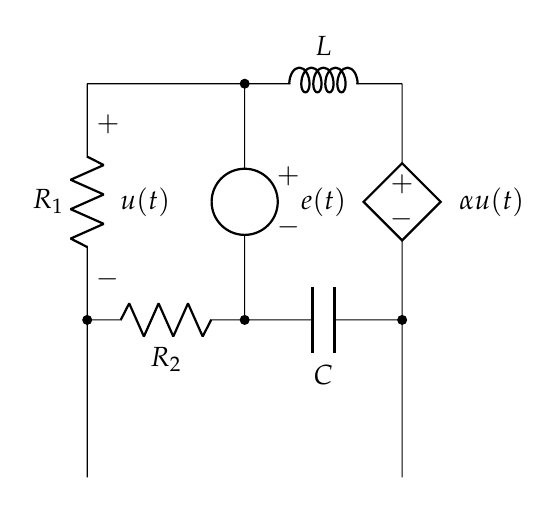
\begin{tikzpicture}
  \coordinate (A) at (0,5);
  \coordinate (B) at (2,5);
  \coordinate (C) at (4,5);
  \coordinate (D) at (0,2);
  \coordinate (E) at (2,2);
  \coordinate (F) at (4,2);
  \coordinate (G) at (0,0);
  \coordinate (H) at (4,0);
  \draw
  (A) to [short, -*] (B)
  to [L, l = $L$] (C)
  (A) to [R, l_= $R_1$, v^= $u(t)$, -*] (D)
  to [R, l_= $R_2$, -*] (E)
  (B) to [esource, v = $e(t)$] (E)
  (C) to [cV, v = $\alpha u(t)$] (F)
  (E) to [C, -*, l_= $C$] (F)
  (D) to [short] (G)
  to [open] (H)
  to [short] (F);
\end{tikzpicture}
\end{document}